\chapter{MATERIAL E MÉTODOS}\label{cap3MatMet}
Neste capítulo, são apresentadas as tecnologias utilizadas, as ferramentas adotadas e as etapas envolvidas no desenvolvimento do Sistema Integrado de Gestão para marmorarias. O objetivo é descrever de forma clara e estruturada o processo de concepção, implementação e validação do ERP, evidenciando as decisões técnicas que orientaram o desenvolvimento da solução. A proposta baseia-se na criação de uma aplicação moderna, acessível e orientada à eficiência operacional, buscando atender às demandas reais do setor de rochas ornamentais.

O desenvolvimento do sistema foi fundamentado em práticas contemporâneas de engenharia de software, com ênfase em modularidade, escalabilidade, desempenho, reuso de componentes e segurança da informação. Para isso, foram selecionadas tecnologias amplamente consolidadas no mercado e compatíveis com uma arquitetura flexível, preparada para evoluções futuras. Além disso, buscou-se garantir uma experiência fluida e intuitiva para os usuários, considerando princípios de usabilidade, padronização de fluxos e redução de fricções no uso diário da aplicação.

A escolha por computação em nuvem e conteinerização teve como objetivo reduzir a manutenção manual de servidores, padronizar ambientes e manter custos operacionais baixos. A arquitetura foi desenhada para que a API e o PostgreSQL executem em contêineres Docker em uma máquina virtual na Google Cloud (Compute Engine) ou em um VPS equivalente --- com manifestos de Kubernetes já preparados no repositório para cenários de maior escala (Seção~\ref{sec:workflow-deploy}) ---, o frontend seja publicado na Vercel, as mídias sejam armazenadas por um backend próprio (local por padrão, com o mesmo contrato de URLs assinadas podendo apontar para o Google Cloud Storage ou para um serviço \textit{S3-compatible} como o Cloudflare R2) e as imagens Docker da API sejam versionadas no GHCR. Por se tratar de um MVP acadêmico, e com o objetivo de manter o material documentado neste trabalho sempre acessível e sob controle de custo, a validação prática do sistema foi conduzida em ambiente Docker local, reproduzindo os mesmos contêineres e a mesma configuração previstos para essa camada de infraestrutura em nuvem. Esse conjunto de decisões permitiu concentrar esforços no desenvolvimento das funcionalidades principais do ERP, criando uma solução robusta, segura e economicamente viável.

Este capítulo também apresenta os princípios que guiaram a modelagem dos processos internos, a definição dos fluxos de informação, as estratégias de persistência de dados e os mecanismos de autenticação utilizados. O intuito é fornecer uma visão detalhada do percurso técnico do projeto, desde as primeiras decisões de arquitetura até as etapas finais de entrega e testes do sistema.

\section{Tecnologias Utilizadas}
O desenvolvimento do ERP para marmorarias baseou-se em tecnologias modernas e amplamente reconhecidas no setor de software, buscando garantir uma experiência eficiente, segura e acessível para os usuários finais. A seleção das ferramentas considerou critérios como facilidade de implementação, agilidade, compatibilidade entre plataformas, escalabilidade e aderência às boas práticas do mercado. A seguir, são listadas as principais tecnologias utilizadas durante o desenvolvimento do projeto.

\begin{itemize}
\item \textbf{Cursor (IDE):} ambiente de desenvolvimento com assistência de Inteligência Artificial contextual, utilizado para acelerar a escrita de código, refatorações e manutenção da consistência arquitetural do projeto.
\item \textbf{Frontend:} Next.js (App Router), React, TypeScript e Tailwind CSS, com comunicação HTTP via Axios e tipagem estática para reduzir erros em tempo de desenvolvimento.
\item \textbf{Backend:} linguagem Go, \textit{framework} Gin para HTTP e GORM como ORM para persistência no PostgreSQL. Autenticação com JWT (\textit{access token} e \textit{refresh token}) e senhas com bcrypt.
\item \textbf{Banco de Dados:} PostgreSQL 15, escolhido por robustez, propriedades ACID e adequação a dados relacionais de clientes, produtos e orçamentos.
\item \textbf{Infraestrutura e Deploy:} Docker e Docker Compose para execução local da API e do banco, reproduzindo a topologia prevista para produção; arquitetura preparada para Google Cloud Compute Engine ou VPS (VM) e para orquestração via Kubernetes (manifestos versionados no repositório); Vercel para o frontend; GHCR para imagens Docker da API; armazenamento de mídias (logo, avatar e produtos) via URLs assinadas, com backend local por padrão e suporte pronto para Google Cloud Storage ou um serviço \textit{S3-compatible} (Cloudflare R2); CI/CD com GitHub Actions (build e publicação de imagem).
\item \textbf{Ferramentas complementares:} Docker, GitHub, Postman (validação de rotas) e a landing page institucional (Next.js) para marketing e captura de leads.
\end{itemize}

\section{Etapas do Desenvolvimento}
O desenvolvimento do sistema ERP para marmorarias foi estruturado em etapas progressivas, iniciando pelo planejamento inicial e avançando pela definição da arquitetura, implementação das funcionalidades e validação do protótipo. A abordagem priorizou modularidade, escalabilidade e segurança, permitindo que o sistema evoluísse de forma consistente ao longo do projeto.

\subsection{Planejamento Inicial}
A etapa de planejamento inicial teve como foco a definição dos objetivos gerais do sistema, a identificação das necessidades operacionais das marmorarias e o levantamento das funcionalidades essenciais para compor a primeira versão do ERP. Nesta fase, foi formulado um MVP, delimitando recursos prioritários como: cadastro multi-\textit{tenant} da empresa, autenticação, gestão de clientes, catálogo de produtos, orçamentos (com status comercial e de obra), configurações da empresa, painel com indicadores e \textit{upload} de imagens.

Além da definição de requisitos, o planejamento envolveu a escolha das tecnologias e o mapeamento dos fluxos de interação do usuário --- login, \textit{provision} da marmoraria, criação de clientes/produtos/orçamentos e atualização de status. Também foram levantados problemas típicos do setor, como fragmentação de informações e baixa previsibilidade de orçamentos, que orientaram o desenho do painel e dos módulos principais.

\subsection{Estruturação da Arquitetura}
A fase de estruturação da arquitetura concentrou-se na organização interna do sistema, incluindo camadas, módulos, estratégias de comunicação e padrões de desenvolvimento. Adotou-se um monólito modular inspirado na \textit{Clean Architecture}, com separação entre domínio, casos de uso, entrega HTTP e infraestrutura.

O backend foi organizado em módulos responsáveis por autenticação, \textit{tenants}, usuários, clientes, produtos, orçamentos, configurações, auditoria, \textit{uploads} e lista de espera (\textit{waitlist}) da landing page. A comunicação com o frontend ocorre por API REST sob o prefixo \texttt{/api/v1}. No frontend, o Next.js (App Router) organiza rotas, componentes e serviços de consumo da API. Na camada de dados, o PostgreSQL e o GORM sustentam o modelo relacional. Versionamento, Docker e pipeline de CI/CD fecham o ciclo de entrega.

\subsection{Desenvolvimento do Backend}

A construção do \textit{backend} teve início com a definição das entidades de domínio que representam o núcleo do sistema de gestão para marmorarias, entre elas: \textit{tenant} (empresa), usuário, cliente, produto, orçamento, configurações, leads da lista de espera e registros de auditoria. A API foi desenvolvida na linguagem Go, utilizando o \textit{framework} Gin para o tratamento de requisições HTTP e o GORM como ORM (\textit{Object-Relational Mapping}) para persistência no banco de dados relacional PostgreSQL.

A organização do código seguiu uma arquitetura em camadas inspirada na \textit{Clean Architecture}, com separação entre domínio (\texttt{domain}), casos de uso (\texttt{usecase}), entrega HTTP (\texttt{delivery/http}) e infraestrutura (\texttt{infra}). Essa divisão permite isolar as regras de negócio das dependências externas, facilitando manutenção, testes e evolução do sistema.

A autenticação foi implementada com base em JWT (\textit{JSON Web Token}), por meio da biblioteca \texttt{golang-jwt}. Após a validação das credenciais, a API emite um par de tokens (\textit{access token} e \textit{refresh token}), contendo \textit{claims} como identificador do usuário, identificador do \textit{tenant}, e-mail, papel (\textit{role}) e permissões. As senhas são armazenadas com hash bcrypt. O fluxo de cadastro de novas empresas ocorre pelo \textit{endpoint} público de \textit{provision}, que cria, em uma única operação, o \textit{tenant}, o usuário administrador e as configurações iniciais da empresa.

Como se trata de uma aplicação \textit{multi-tenant}, cada recurso de negócio é isolado pelo \texttt{tenant\_id} presente no token. \textit{Middlewares} de autenticação, autorização por papel/permissão e auditoria protegem as rotas autenticadas, registrando operações de criação, atualização e exclusão para rastreabilidade.

Foram implementados \textit{endpoints} sob o prefixo \texttt{/api/v1} para:
\begin{itemize}
  \item \textit{Provision} de empresa e administrador, \textit{login}, renovação de token e verificação de e-mail;
  \item Cadastro e gestão de usuários, clientes, produtos e orçamentos;
  \item Configurações da empresa (dados cadastrais e logo);
  \item \textit{Upload} de arquivos (logo, avatar e imagens de produto) via URLs assinadas, emitidas pelo próprio backend de armazenamento (local por padrão);
  \item Consulta de auditoria e exportação básica de relatórios de produtos;
  \item Cadastro público na lista de espera (landing page), persistido no PostgreSQL;
  \item \textit{Healthchecks} (\texttt{/health}, \texttt{/liveness}, \texttt{/readiness}) para monitoramento do ambiente de execução, local ou em nuvem.
\end{itemize}

O armazenamento de mídias foi implementado por trás de uma interface (\texttt{Signer}) com duas implementações intercambiáveis: um backend em disco local, selecionado por padrão, e um backend para o Google Cloud Storage (GCS), habilitado automaticamente quando a variável \texttt{GCS\_BUCKET} é configurada. Ambos seguem o mesmo contrato de \textit{signed URLs} de escrita e leitura, de modo que o restante da aplicação -- e o próprio \textit{frontend} -- não precisa saber qual backend está ativo. O backend local foi adotado como padrão deste trabalho por eliminar a dependência de uma conta de nuvem ativa e qualquer custo operacional durante a avaliação acadêmica, sem abrir mão do mesmo modelo de segurança: o \textit{token} de \textit{upload} é assinado com HMAC-SHA256 e expira em poucos minutos, e o arquivo nunca trafega pelo processo da API além da escrita em disco. Optou-se por manter o próprio GCS como o backend de nuvem já implementado (em vez de substituí-lo por outro serviço) porque o contrato de \textit{signed URLs} já validado neste trabalho é o mesmo adotado por serviços \textit{S3-compatible} de baixo custo, como o Cloudflare R2, tornando essa também uma alternativa viável de baixo custo caso a operação em nuvem seja retomada.

Quando um arquivo precisa ser enviado, o fluxo ocorre da seguinte forma: o cliente autenticado solicita uma URL de \textit{upload} ao \textit{endpoint} \texttt{/uploads/sign}; a API gera a chave do objeto e devolve uma URL assinada de PUT apontando para o backend ativo; o \textit{frontend} realiza o envio direto a essa URL (ao próprio servidor da API, no backend local, ou ao \textit{bucket}, no backend de nuvem); posteriormente, a aplicação persiste apenas a referência (\texttt{object\_key}) e solicita URLs de leitura quando necessário. Com essa abordagem, a arquitetura permanece leve, segura e escalável no tratamento de conteúdos multimídia, independentemente do backend de armazenamento selecionado.
 
\begin{figure}[H]
  \centering
  \captionsetup{justification=centering}
  \caption{Diagrama da arquitetura geral da aplicação.}
  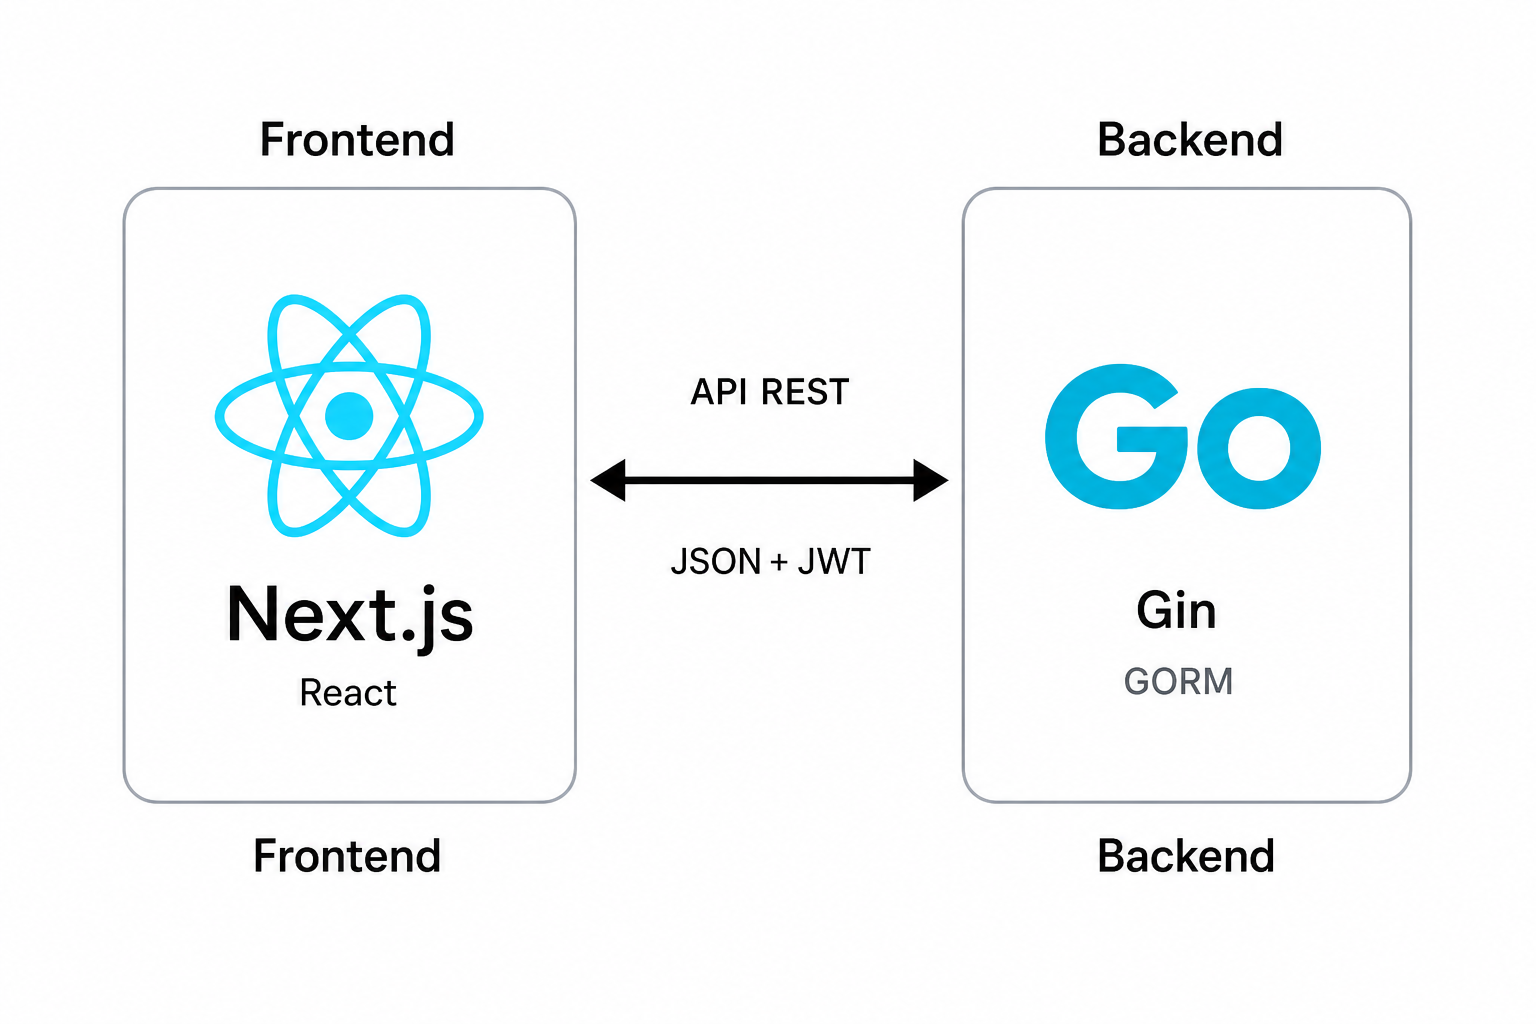
\includegraphics[width=0.85\textwidth]{figures/diagrama-arquitetura-geral.png}
  \label{fig:arquitetura-geral}
\end{figure}
{\centering\small Fonte: O Autor, 2026.\par}
\vspace{0.8em}

\subsection{Desenvolvimento do Frontend}

O desenvolvimento da interface web priorizou usabilidade, responsividade e compatibilidade entre navegadores, permitindo que o usuário gerencie a operação da marmoraria a partir de um painel administrativo. A aplicação foi construída com Next.js, utilizando o App Router baseado em sistema de arquivos. Essa abordagem simplifica a organização das rotas, facilita a navegação entre páginas e favorece a leitura do código, acelerando o ciclo de desenvolvimento.

A tipagem estática com TypeScript e a estilização com Tailwind CSS contribuíram para um código mais seguro e consistente, além de uma interface adaptável a diferentes resoluções de tela. A comunicação com a API REST foi implementada por meio da biblioteca Axios, com interceptores responsáveis por anexar o token JWT às requisições e renovar a sessão de forma silenciosa quando o \textit{access token} expira. Os tokens são persistidos no navegador e utilizados para manter o usuário autenticado entre recarregamentos da página.

As principais funcionalidades implementadas no \textit{frontend} incluem: autenticação (\textit{login} e cadastro/\textit{provision} da empresa), painel inicial com indicadores e gráficos (agregados no navegador a partir das listas da API), gestão de clientes, produtos e orçamentos, edição de perfil, configurações da empresa (dados cadastrais e logo) e controle de acesso por papel/permissão. Componentes reutilizáveis --- formulários, tabelas, \textit{modals}, campos de \textit{upload} e layout do painel --- foram adotados para reduzir duplicação e padronizar a experiência do usuário.

O fluxo de navegação da aplicação é apresentado na Figura~\ref{fig:estrutura-navegacao-app-router}. Após o acesso inicial, o usuário realiza autenticação; em seguida, é direcionado ao \textit{dashboard}, de onde pode navegar para os módulos de clientes, produtos, orçamentos e configurações.
 
\begin{figure}[H]
  \centering
  \captionsetup{justification=centering}
  \caption{Estrutura de navegação via App Router.}
  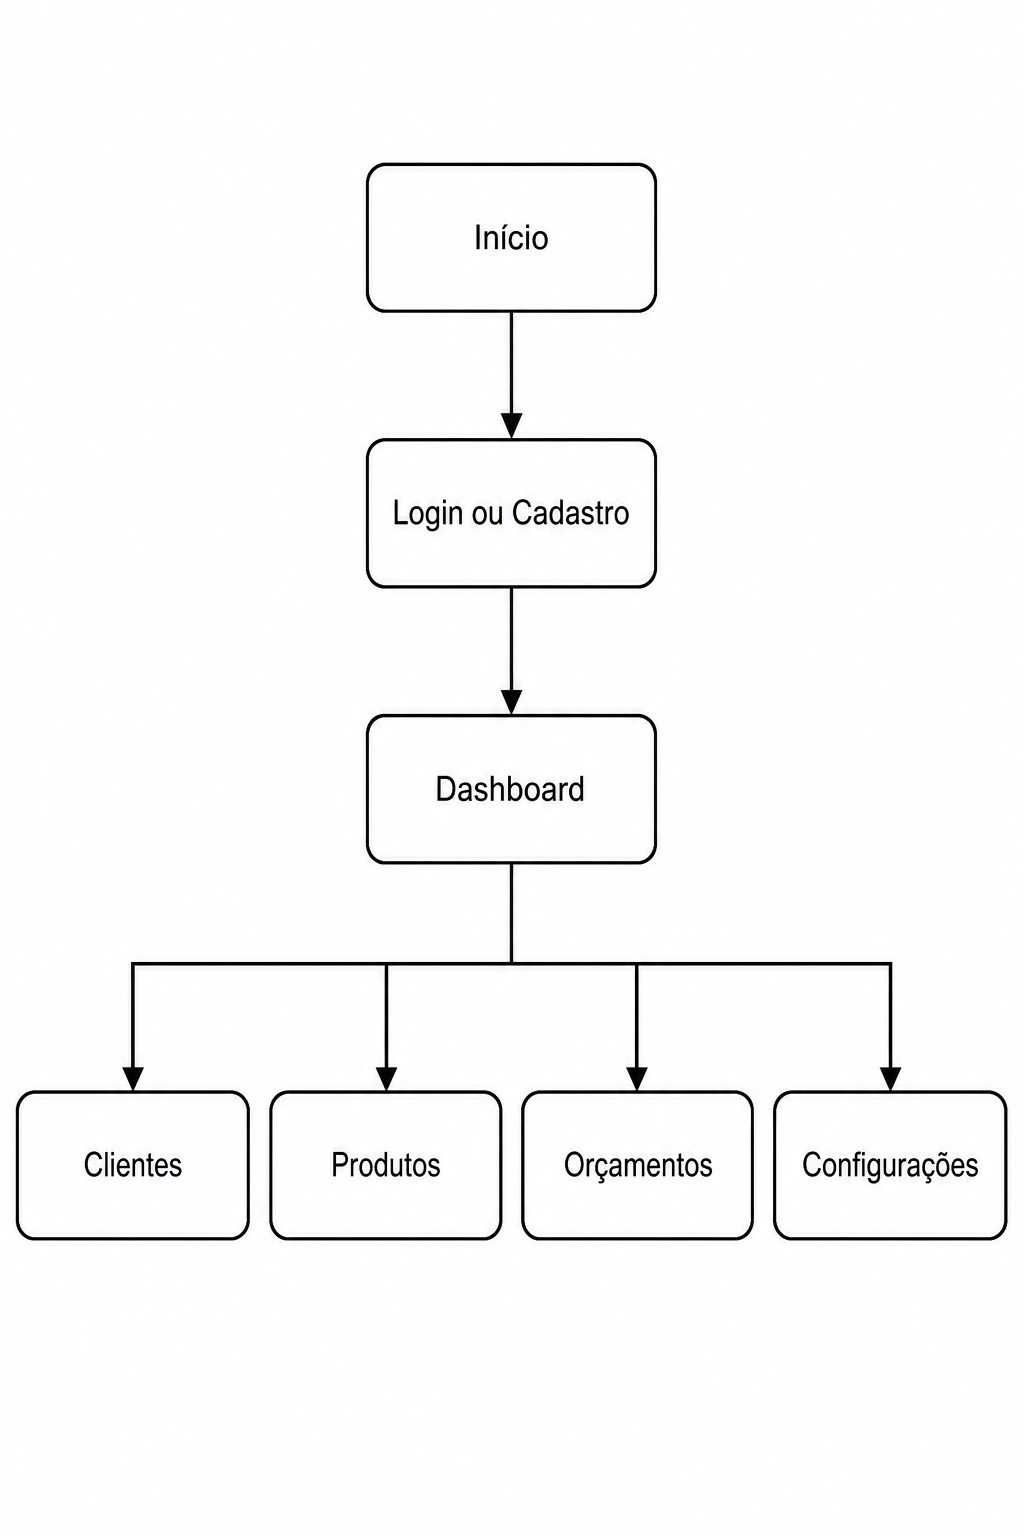
\includegraphics[width=0.85\textwidth]{figures/estrutura-navegacao-app-router.png}
  \label{fig:estrutura-navegacao-app-router}
\end{figure}
{\centering\small Fonte: O Autor, 2026.\par}
\vspace{0.8em}

\subsection{Integração entre Camadas}

A integração entre o \textit{frontend} e o \textit{backend} foi realizada de forma progressiva, permitindo validar funcionalidades essenciais como autenticação (\textit{login}), cadastro de empresa (\textit{provision}), gestão de clientes, produtos e orçamentos, além das configurações da empresa. A comunicação ocorre por meio de requisições HTTP enviadas pelo painel web à API REST, utilizando tokens JWT para autenticação e autorização. No \textit{frontend}, a biblioteca Axios é responsável por essas requisições; por meio de \textit{interceptors}, o token de acesso é anexado automaticamente ao cabeçalho \texttt{Authorization} e, em caso de expiração (resposta HTTP 401), a sessão é renovada de forma silenciosa com o \textit{refresh token}, centralizando também o tratamento de erros.

A Figura~\ref{fig:fluxo-cliente-servidor} ilustra o fluxo de comunicação entre cliente e servidor. O cliente envia uma requisição HTTP contendo o cabeçalho JWT; o servidor processa a solicitação e devolve uma resposta HTTP com \textit{payload} em JSON.

\begin{figure}[H]
  \centering
  \captionsetup{justification=centering}
  \caption{Fluxo de comunicação cliente-servidor.}
  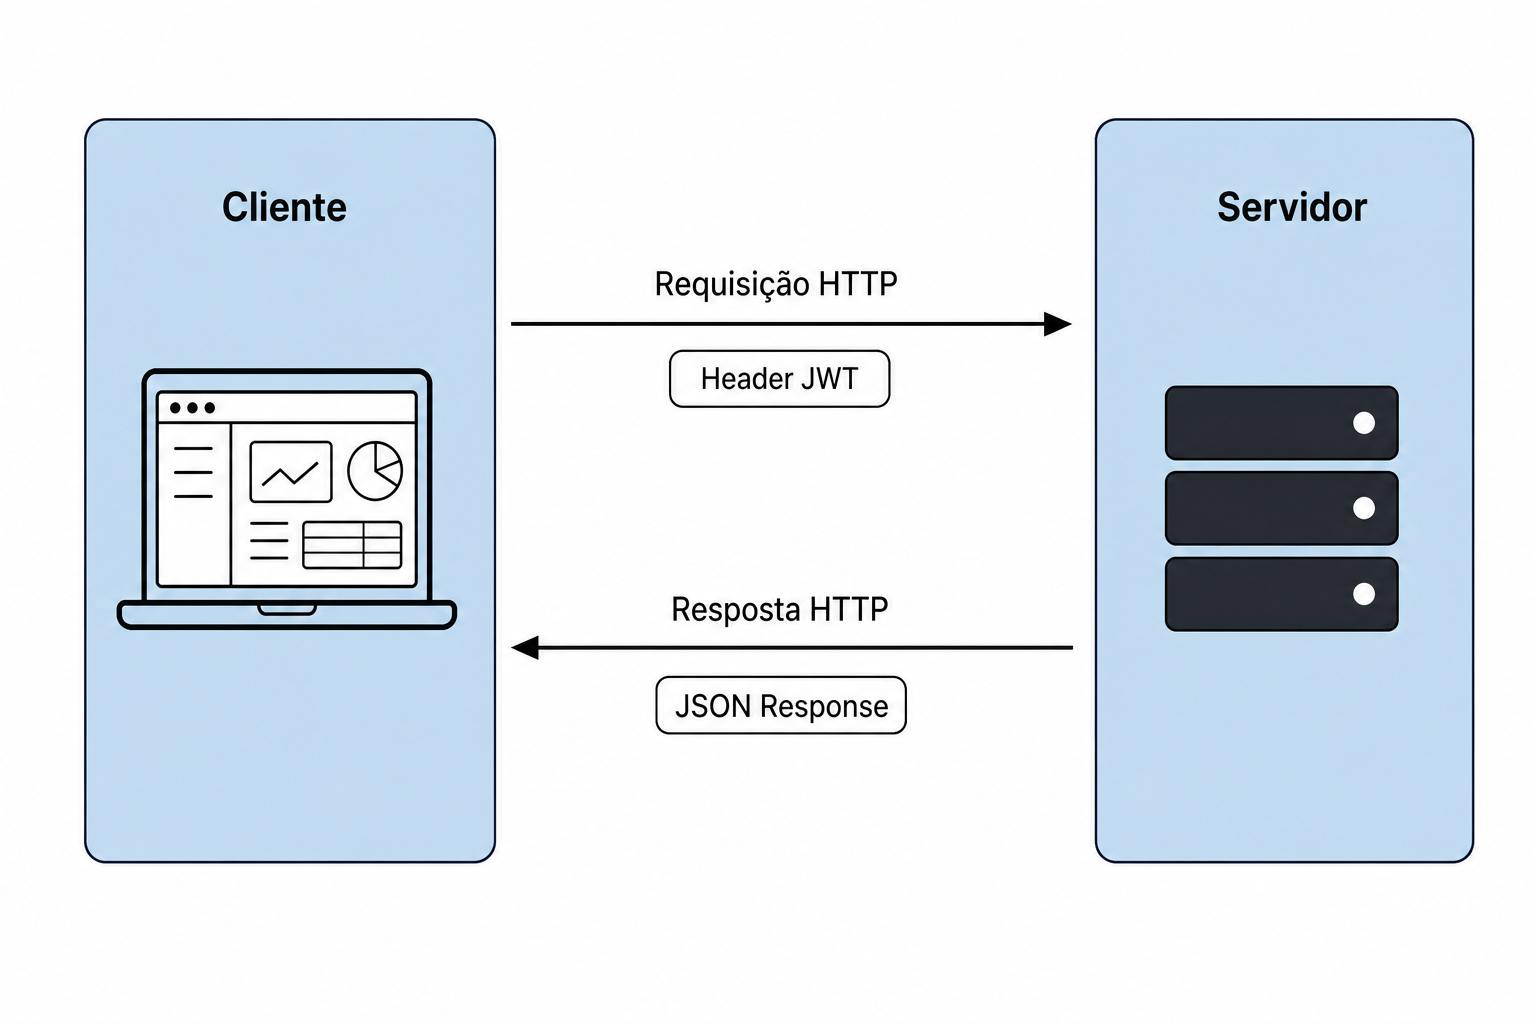
\includegraphics[width=0.85\textwidth]{figures/cliente-servidor.png}
  \label{fig:fluxo-cliente-servidor}
\end{figure}
{\centering\small Fonte: O Autor, 2026.\par}
\vspace{0.8em}

No que se refere a arquivos (logo da empresa e imagens de produtos), o \textit{frontend} e o \textit{backend} atuam de forma coordenada: o painel solicita à API uma URL assinada de \textit{upload}, envia o arquivo diretamente ao backend de armazenamento ativo (local por padrão, ou ao \textit{bucket} de nuvem quando configurado) e, em seguida, persiste apenas a referência do objeto (\texttt{object\_key}) nos dados da aplicação. Para exibição, o cliente solicita uma URL de leitura. Essa estratégia reduz a carga sobre a API e garante consistência entre os dados cadastrais e os arquivos multimídia apresentados ao usuário, sem que o \textit{frontend} precise conhecer qual backend está ativo.

\subsection{Testes e Validação}
\label{sec:testes-e-validacao-cap3}

Durante o desenvolvimento, a validação do sistema combinou testes manuais da interface web e testes automatizados no \textit{backend}, com foco em regras de negócio, autenticação e consistência das respostas da API.

No \textit{frontend}, foram realizados testes manuais em navegadores desktop e em dispositivos móveis (iPhone e Android), avaliando a responsividade do painel, o fluxo de autenticação (\textit{login}, renovação de sessão e redirecionamento para rotas protegidas), a navegação entre os módulos (clientes, produtos, orçamentos e configurações) e a consistência dos dados exibidos após as operações de criação e edição. Também foram verificados cenários de \textit{upload} de imagens (logo e produtos), incluindo a obtenção de URLs assinadas e a exibição correta dos arquivos gravados pelo backend de armazenamento local.

No \textit{backend}, a validação automatizada foi implementada com o pacote padrão \texttt{testing} da linguagem Go, executada por meio do comando \texttt{go test ./...}. Para isolar as regras de negócio das dependências de infraestrutura, foram utilizados \textit{mocks} manuais de repositórios (implementações em memória das interfaces de domínio), localizados no pacote \texttt{internal/mocks}. Essa abordagem permite simular o comportamento de persistência sem a necessidade de banco de dados real durante os testes unitários. Dentre os cenários cobertos pelos testes automatizados, destacam-se:
\begin{itemize}
  \item autenticação e emissão/validação de tokens JWT, incluindo geração de \textit{access token} e \textit{refresh token};
  \item hashing e verificação de senhas com bcrypt;
  \item \textit{provision} de \textit{tenant} com criação do usuário administrador e associação ao plano selecionado;
  \item validação de documentos (CNPJ), incluindo normalização de máscaras e rejeição de valores inválidos;
  \item \textit{middleware} de autenticação e autorização por papel (\textit{role}), utilizando \texttt{httptest} e contexto de teste do Gin.
\end{itemize}

Complementarmente, foram realizadas validações manuais dos principais \textit{endpoints} da API (via Postman e pelo próprio painel), conferindo status HTTP, estrutura do JSON de resposta, mensagens de erro e regras de autorização.

Essa combinação de testes manuais e automatizados permitiu verificar a corretude das regras de negócio, a integridade das requisições autenticadas e a estabilidade dos fluxos críticos do sistema na versão avaliada neste trabalho.

\section{Funcionalidades da Aplicação}

O aplicativo Onmarmoraria foi criado com o objetivo de facilitar a vida de pequenas marmorarias por meio de uma interface moderna, intuitiva e amigável. A plataforma busca centralizar dados operacionais e apoiar decisões com base em indicadores do painel, priorizando usabilidade e segurança dos dados na nuvem. A seguir, estão descritas as funcionalidades atualmente implementadas, começando pela landing page de marketing e, em seguida, pelo painel administrativo.

\subsection{Landing page institucional}

Antes do acesso ao painel, o projeto conta com uma landing page voltada ao marketing do Onmarmoraria. Essa página apresenta a proposta de valor do ERP, funcionalidades previstas e um formulário de lista de espera. O objetivo é comunicar o produto a marmorarias e coletar informações de contato e perfil operacional (porte e volume de orçamentos), armazenadas no banco de dados do backend. A Figura~\ref{fig:landing-page} ilustra a página.

\subsection{Tela Inicial de Login}

A primeira tela da aplicação apresenta o formulário de \textit{login}, guiando o fluxo inicial de navegação. Nesta fase de desenvolvimento descrita no presente capítulo, a tela também oferecia um atalho de criação de conta da marmoraria (\textit{provision}) diretamente pelo painel, ilustrado na Figura~\ref{fig:login-page}. Conforme discutido no Capítulo~\ref{cap5Discussao}, esse atalho de autoatendimento foi posteriormente removido, por não corresponder ao modelo de operação pretendido para o produto.

\begin{figure}[H]
  \centering
  \captionsetup{justification=centering}
  \caption{Tela inicial com opções de Login e Criar Conta (versão anterior à revisão de escopo descrita no Capítulo~\ref{cap5Discussao}).}
  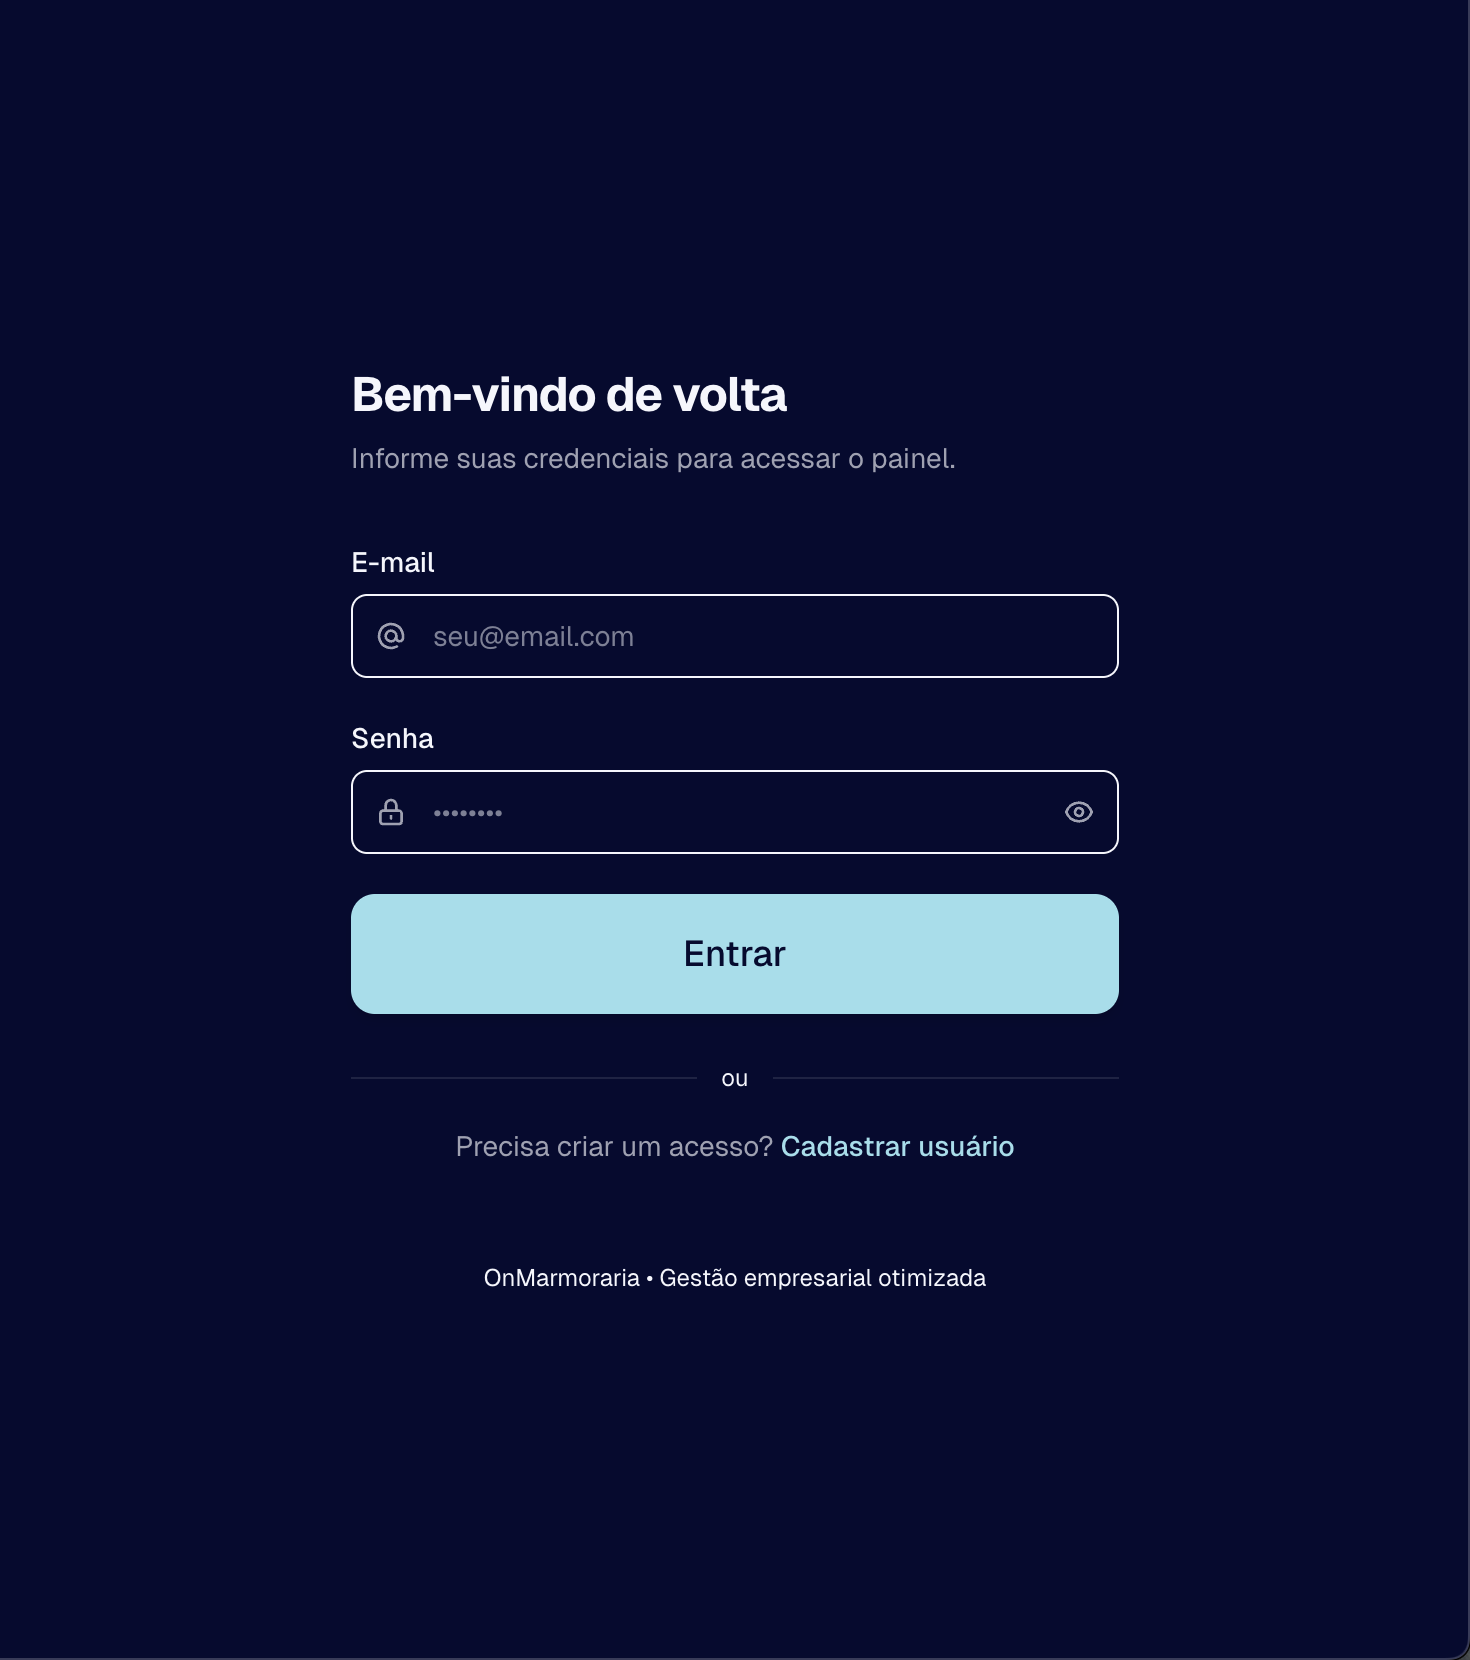
\includegraphics[width=0.85\textwidth]{figures/login-page.png}
  \label{fig:login-page}
\end{figure}
{\centering\small Fonte: O Autor, 2026.\par}
\vspace{0.8em}

Na versão atual do sistema, a tela de login foi simplificada, sem o atalho de autoatendimento discutido acima, conforme ilustrado na Figura~\ref{fig:login-atual} (desktop) e na Figura~\ref{fig:login-mobile} (dispositivo móvel), essa última também evidenciando a responsividade do formulário de autenticação.

\begin{figure}[H]
  \centering
  \captionsetup{justification=centering}
  % TODO(Marcelo): substituir o \fbox abaixo por
  % \includegraphics[width=0.85\textwidth]{figures/login-atual.png}
  \fbox{\parbox[c][6cm][c]{0.85\textwidth}{\centering\itshape [Espaço reservado -- print: tela de login atual (desktop), sem o atalho de criação de conta]}}
  \caption{Tela de login na versão atual do sistema (desktop).}
  \label{fig:login-atual}
\end{figure}
{\centering\small Fonte: O Autor, 2026.\par}
\vspace{0.8em}

\begin{figure}[H]
  \centering
  \captionsetup{justification=centering}
  % TODO(Marcelo): substituir o \fbox abaixo por
  % \includegraphics[width=0.5\textwidth]{figures/login-mobile.png}
  \fbox{\parbox[c][6cm][c]{0.5\textwidth}{\centering\itshape [Espaço reservado -- print: tela de login aberta no iPhone/Android]}}
  \caption{Tela de login renderizada em viewport de \textit{smartphone}.}
  \label{fig:login-mobile}
\end{figure}
{\centering\small Fonte: O Autor, 2026.\par}
\vspace{0.8em}

\subsection{Criação de Conta (\textit{Provision} da Empresa)}

O \textit{provision} cria a marmoraria e o usuário administrador em uma única operação. São solicitados: nome da empresa, CNPJ (opcional, com validação), nome do administrador, e-mail e senha (mínimo de oito caracteres). Em caso de sucesso, o sistema autentica o usuário e redireciona ao \textit{dashboard}; quando a verificação de e-mail está habilitada, é exibida mensagem orientando a confirmação do endereço informado. Na versão atual do sistema, essa operação é acionada pelo operador da plataforma diretamente via API, e não mais por uma tela de autoatendimento público (Capítulo~\ref{cap5Discussao}).

\subsection{Dashboard}

A tela de \textit{dashboard} apresenta as principais métricas a serem analisadas. Esses indicadores são calculados no \textit{frontend} a partir dos orçamentos e clientes retornados pela API (não há endpoint dedicado de analytics). Entre elas:

\begin{itemize}
    \item Orçamentos do mês;
    \item Taxa de conversão;
    \item Faturamento estimado;
    \item Ticket médio;
    \item Gráfico de orçamentos nos últimos 30 dias;
    \item Gráfico de barras comparando aprovados e rejeitados nos últimos meses;
    \item Clientes mais recentes / novos clientes no mês;
    \item Top 5 clientes por valor orçado.
\end{itemize}

\begin{figure}[H]
  \centering
  \captionsetup{justification=centering}
  \caption{Painel inicial (dashboard) com indicadores e gráficos.}
  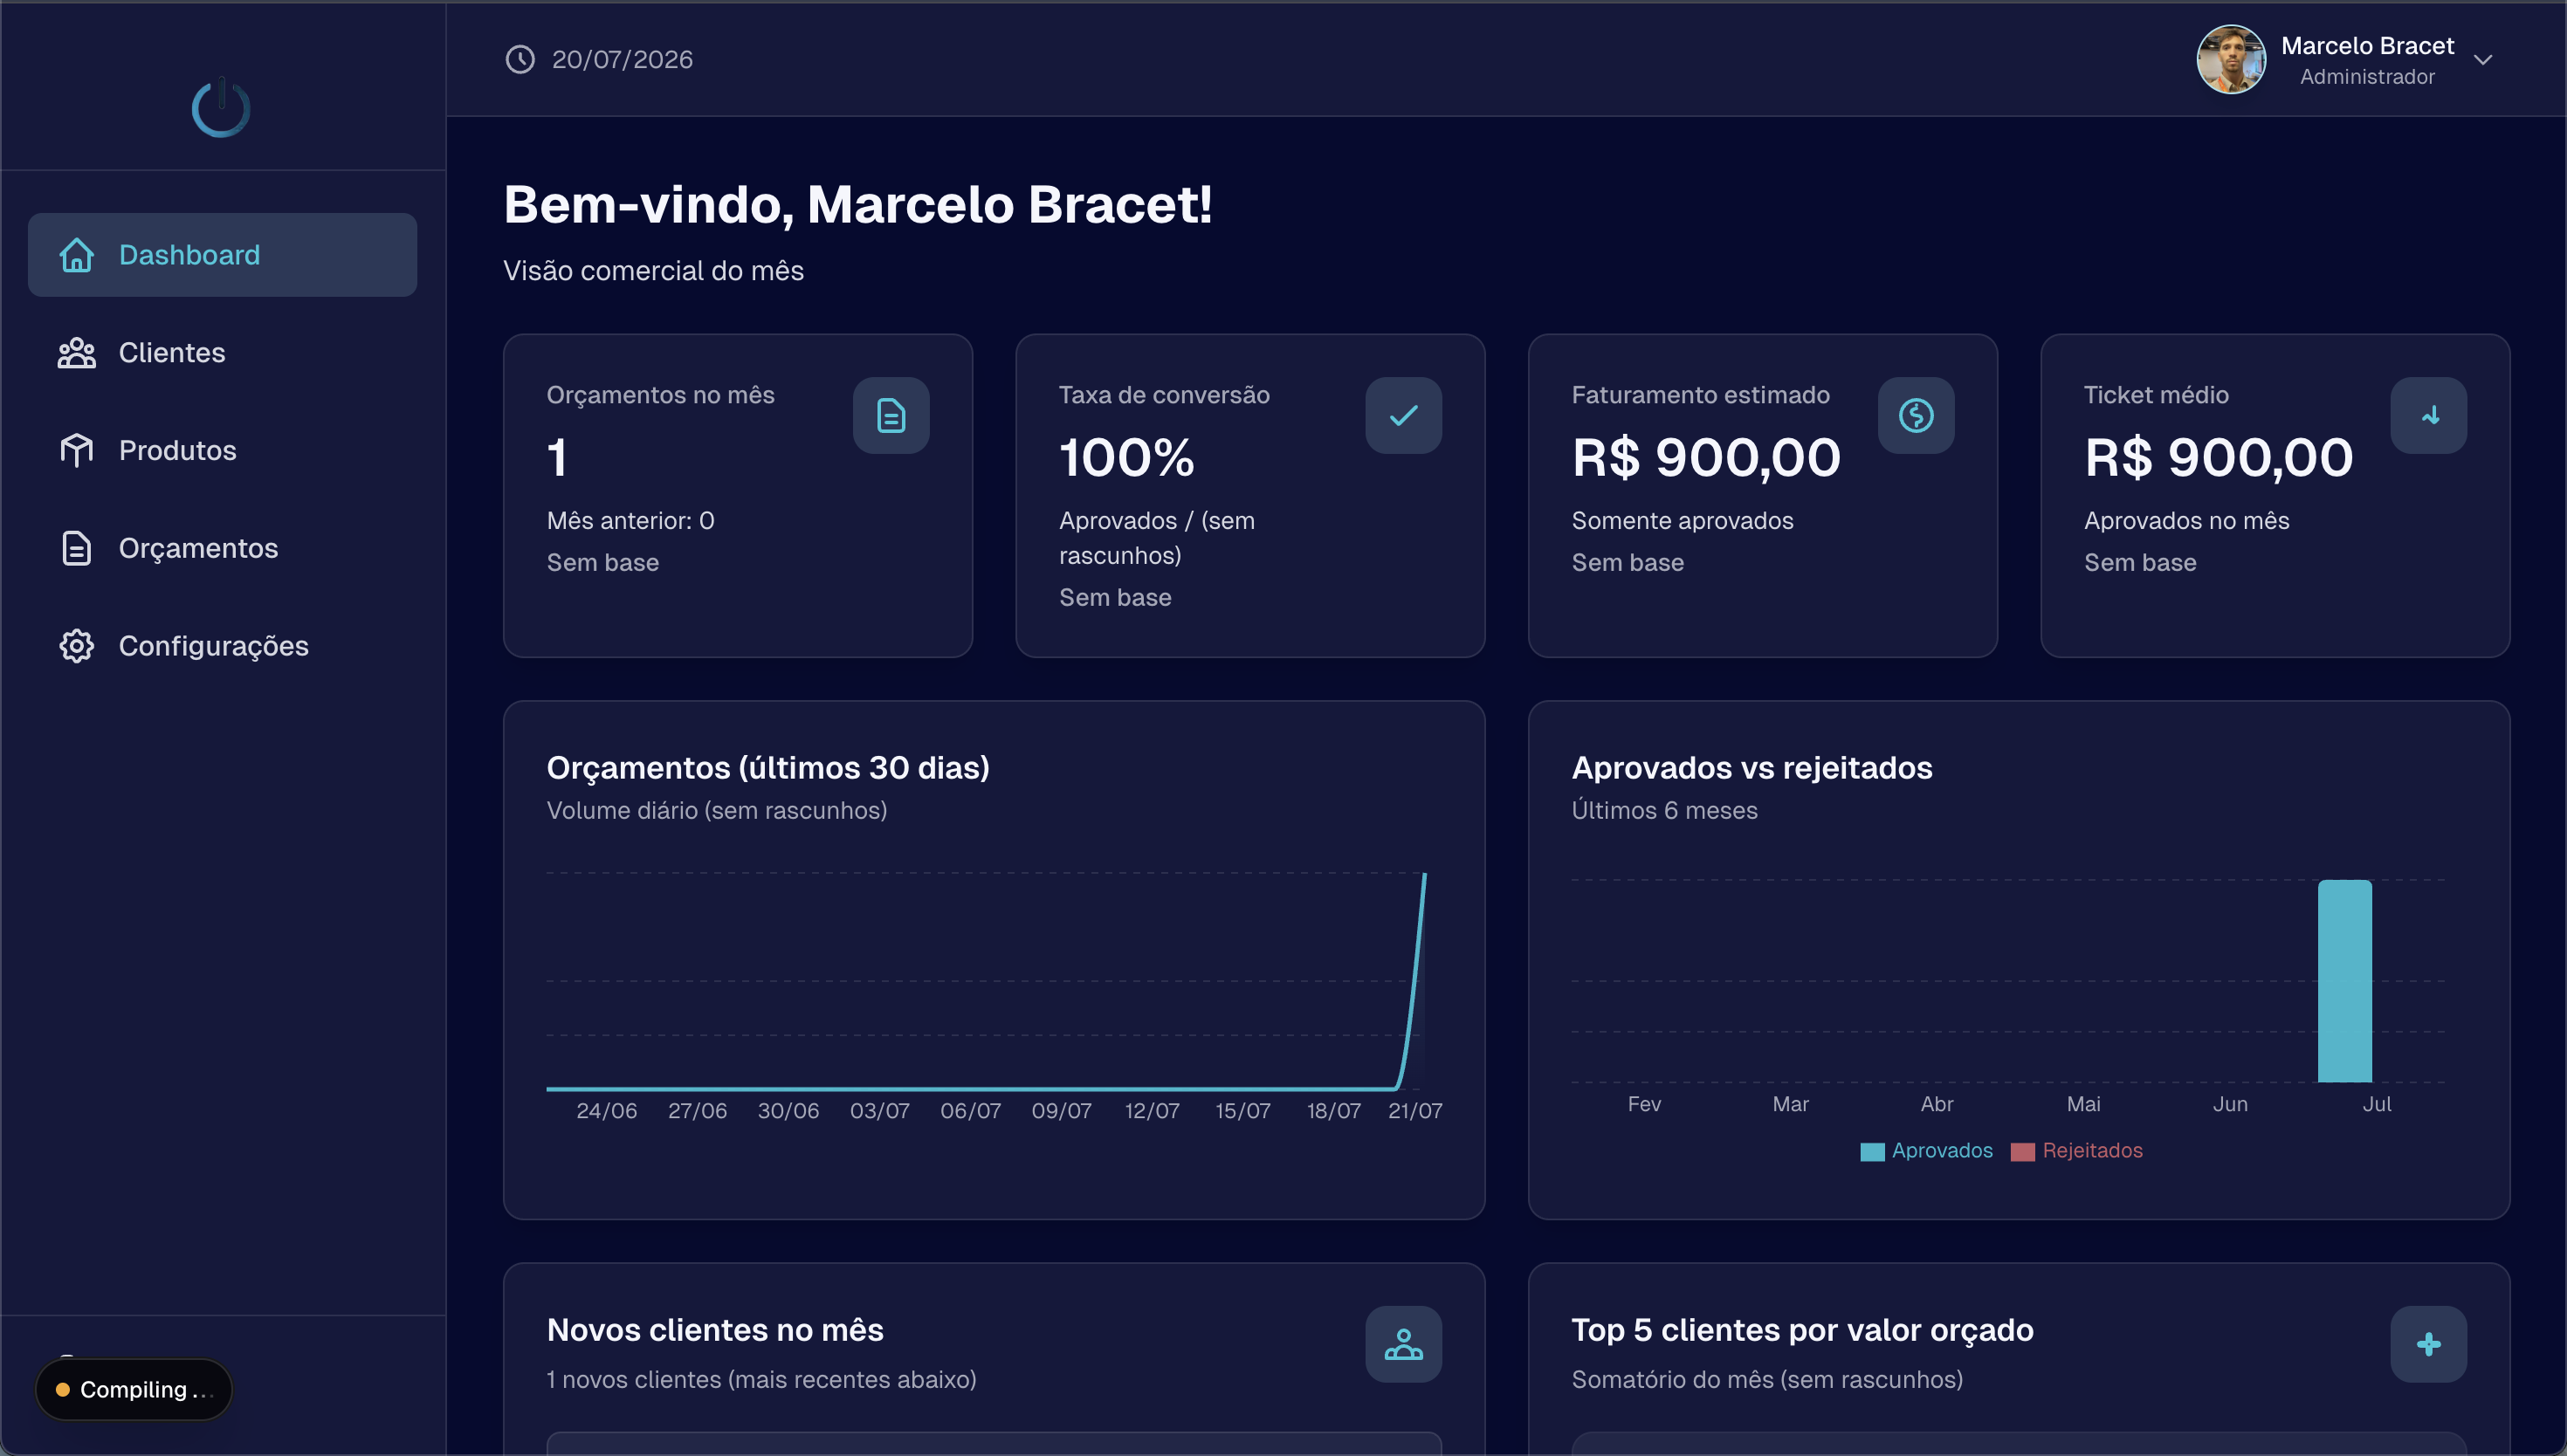
\includegraphics[width=0.95\textwidth]{figures/dashboard.png}
  \label{fig:dashboard}
\end{figure}
{\centering\small Fonte: O Autor, 2026.\par}
\vspace{0.8em}

\begin{figure}[H]
  \centering
  \captionsetup{justification=centering}
  \caption{Continuação do dashboard com listagens e rankings.}
  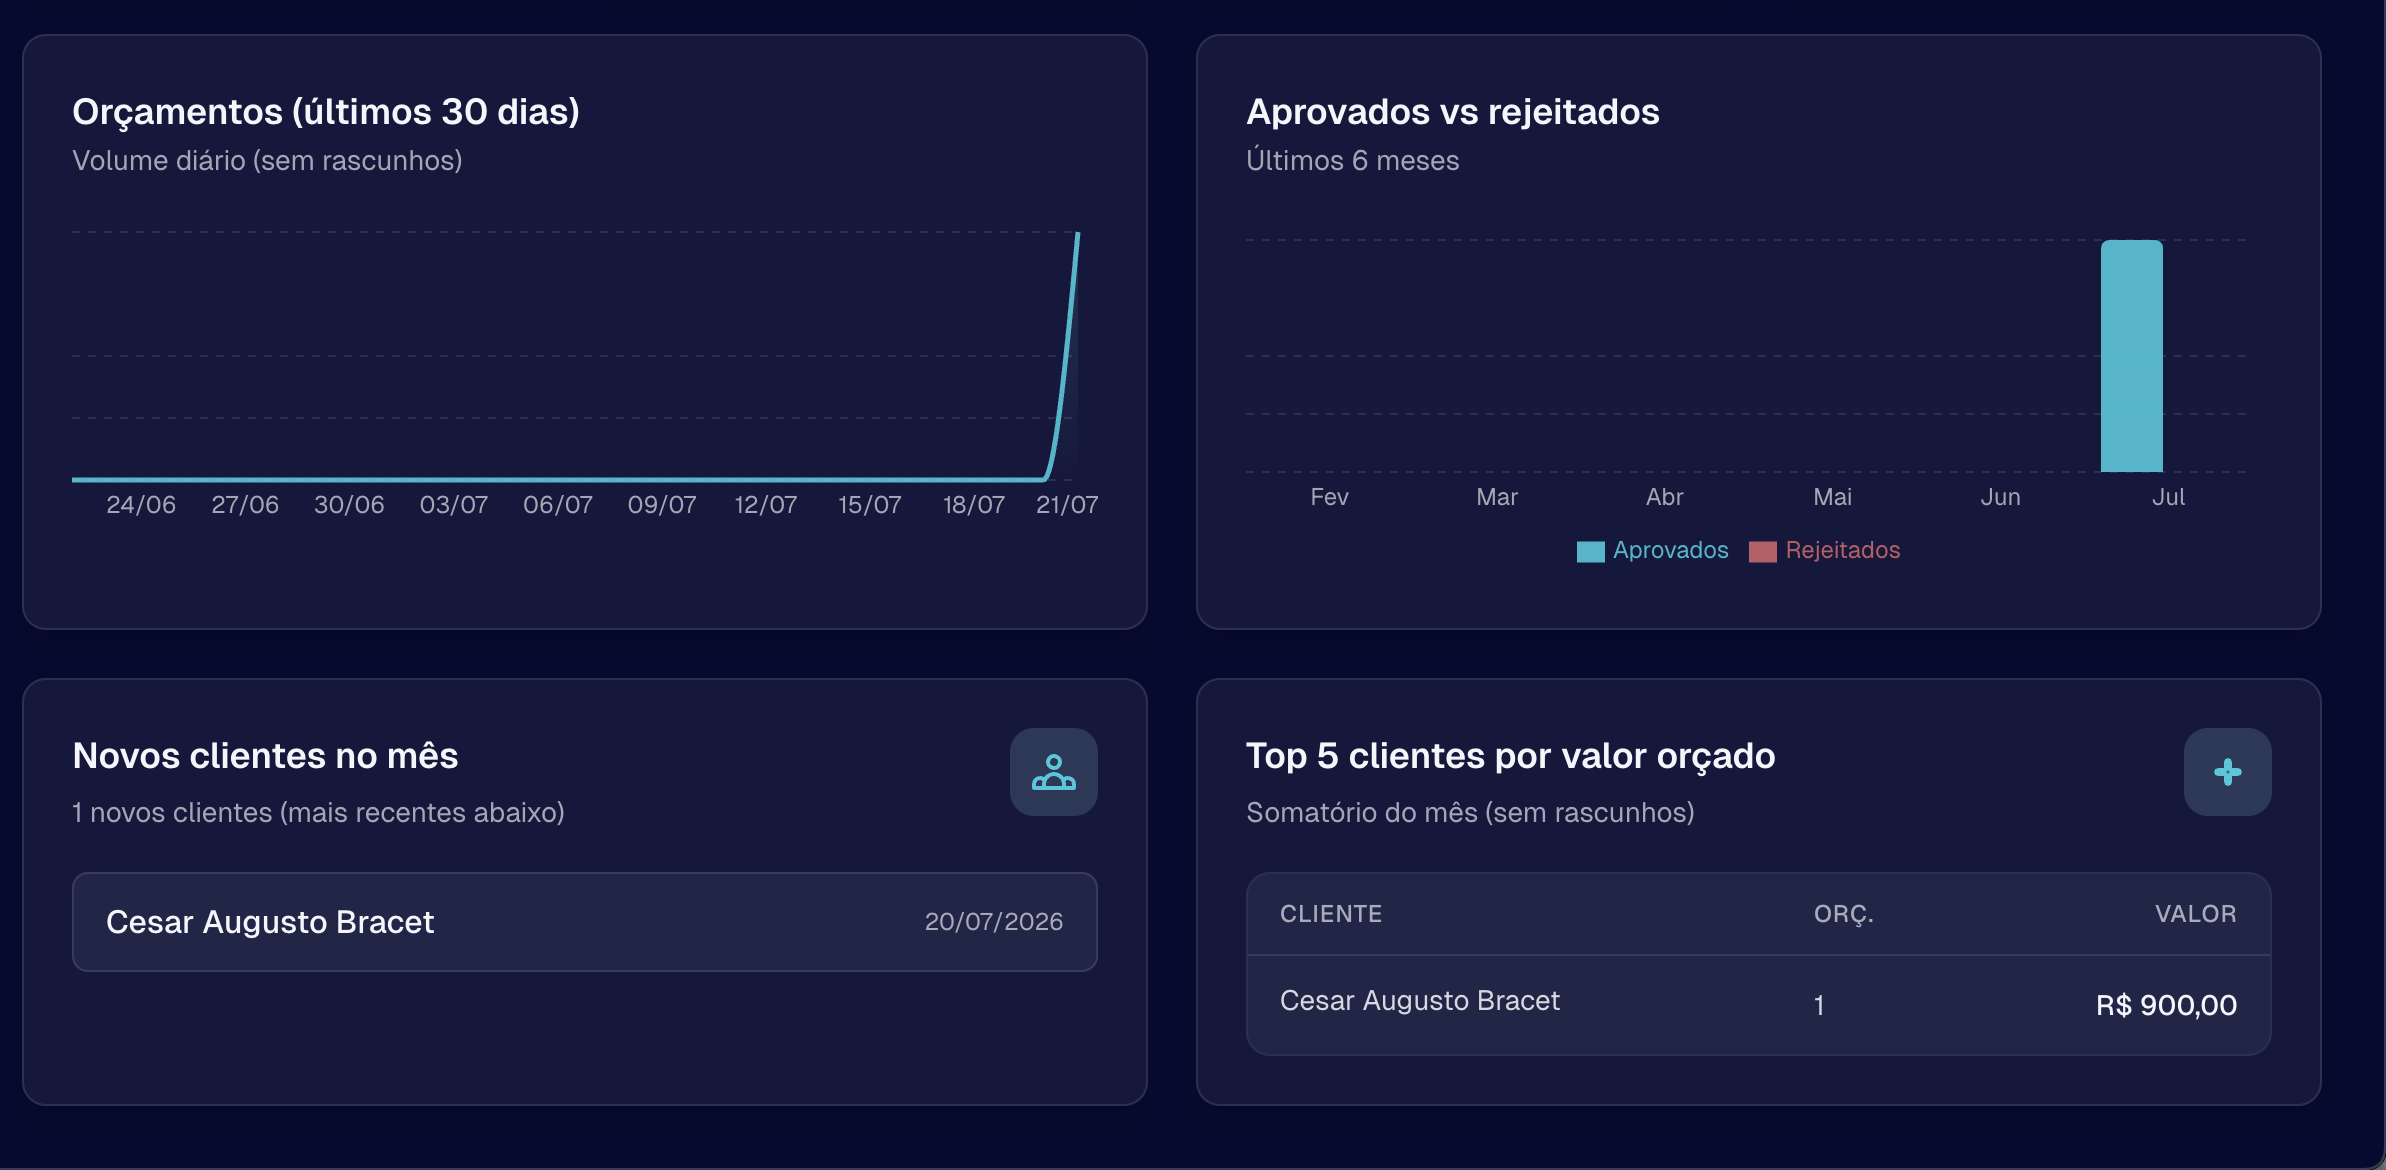
\includegraphics[width=0.95\textwidth]{figures/continuacao-dashboard.png}
  \label{fig:dashboard-cont}
\end{figure}
{\centering\small Fonte: O Autor, 2026.\par}
\vspace{0.8em}

\subsection{Gestão de Clientes}

O módulo de clientes permite listar, criar, editar e excluir registros vinculados ao \textit{tenant}. O formulário contempla nome, e-mail, telefone, documento (CPF ou CNPJ), endereço, cidade, UF e CEP, com validações no frontend e regras no backend. A partir da listagem, o usuário pode abrir o formulário de novo cliente e, após o salvamento, o registro passa a constar na grade.
\begin{figure}[H]
  \centering
  \captionsetup{justification=centering}
  % TODO(Marcelo): substituir o \fbox abaixo por
  % \includegraphics[width=0.85\textwidth]{figures/clientes.png}
  \fbox{\parbox[c][6cm][c]{0.85\textwidth}{\centering\itshape [Espaço reservado -- print: listagem do módulo Clientes, com cliente de teste cadastrado]}}
  \caption{Módulo de gestão de clientes: listagem de registros do \textit{tenant} (dado fictício de teste).}
  \label{fig:clientes}
\end{figure}
{\centering\small Fonte: O Autor, 2026.\par}
\vspace{0.8em}


\subsection{Produtos e Orçamentos}

O módulo de produtos permite cadastrar o catálogo da marmoraria, inclusive com imagem armazenada pelo backend de armazenamento de mídias. O módulo de orçamentos permite criar e editar propostas vinculadas a clientes e itens, com atualização de status comercial e de obra, além de visualização/impressão. Esses fluxos constituem o núcleo operacional do MVP entregue neste trabalho.
\begin{figure}[H]
  \centering
  \captionsetup{justification=centering}
  % TODO(Marcelo): substituir o \fbox abaixo por
  % \includegraphics[width=0.85\textwidth]{figures/produtos.png}
  \fbox{\parbox[c][6cm][c]{0.85\textwidth}{\centering\itshape [Espaço reservado -- print: listagem do módulo Produtos]}}
  \caption{Módulo de catálogo de produtos.}
  \label{fig:produtos}
\end{figure}
{\centering\small Fonte: O Autor, 2026.\par}
\vspace{0.8em}

\begin{figure}[H]
  \centering
  \captionsetup{justification=centering}
  % TODO(Marcelo): substituir o \fbox abaixo por
  % \includegraphics[width=0.85\textwidth]{figures/orcamentos.png}
  \fbox{\parbox[c][6cm][c]{0.85\textwidth}{\centering\itshape [Espaço reservado -- print: listagem do módulo Orçamentos (dado fictício de teste)]}}
  \caption{Módulo de gestão de orçamentos, com filtro por status.}
  \label{fig:orcamentos}
\end{figure}
{\centering\small Fonte: O Autor, 2026.\par}
\vspace{0.8em}


\subsection{Configurações e Perfil}

Nas configurações, o administrador atualiza dados cadastrais da empresa e o logo (via \textit{upload} assinado pelo backend de armazenamento) e gerencia usuários do \textit{tenant}. No perfil, o usuário pode atualizar informações pessoais e avatar. Não há bloqueio por plano ou gateway de pagamento nesta versão do MVP.

\subsection{Responsividade em Dispositivos Móveis}

Para além dos testes descritos na Seção~\ref{sec:testes-e-validacao-cap3}, o painel foi acessado em navegador a partir de aparelhos físicos iPhone e Android, na mesma rede local do ambiente de desenvolvimento, permitindo observar o comportamento real de \textit{layout}, toque e navegação em telas de tamanho reduzido. As Figuras~\ref{fig:mobile-dashboard} e \ref{fig:mobile-clientes} ilustram o painel renderizado em viewport de \textit{smartphone}.

\begin{figure}[H]
  \centering
  \captionsetup{justification=centering}
  % TODO(Marcelo): substituir o \fbox abaixo por
  % \includegraphics[width=0.85\textwidth]{figures/mobile-dashboard.png}
  \fbox{\parbox[c][6cm][c]{0.85\textwidth}{\centering\itshape [Espaço reservado -- print: dashboard aberto no iPhone/Android]}}
  \caption{Painel (dashboard) renderizado em viewport de \textit{smartphone}.}
  \label{fig:mobile-dashboard}
\end{figure}
{\centering\small Fonte: O Autor, 2026.\par}
\vspace{0.8em}

\begin{figure}[H]
  \centering
  \captionsetup{justification=centering}
  % TODO(Marcelo): substituir o \fbox abaixo por
  % \includegraphics[width=0.85\textwidth]{figures/mobile-clientes.png}
  \fbox{\parbox[c][6cm][c]{0.85\textwidth}{\centering\itshape [Espaço reservado -- print: listagem de clientes aberta no iPhone/Android]}}
  \caption{Módulo de clientes renderizado em viewport de \textit{smartphone}.}
  \label{fig:mobile-clientes}
\end{figure}
{\centering\small Fonte: O Autor, 2026.\par}
\vspace{0.8em}

\section{Integrações externas}

Para complementar as funcionalidades principais, o Onmarmoraria utiliza serviços externos de armazenamento e, opcionalmente, de pagamento.

\subsection{Armazenamento de Imagens: Backend Local e GCS/R2 Opcionais}

O armazenamento de logo da empresa, avatar de usuários e imagens de produtos é resolvido, por padrão, por um backend próprio em disco local (\texttt{internal/infra/storage/local}): a API assina um \textit{token} de \textit{upload} com expiração curta (HMAC-SHA256) e o navegador envia o arquivo diretamente ao próprio servidor da API, que grava em disco e serve o arquivo de volta por uma rota estática. Quando a variável \texttt{GCS\_BUCKET} é preenchida, o mesmo \textit{endpoint} de assinatura passa a emitir URLs de PUT/GET (esquema V4) contra um \textit{bucket} privado do Google Cloud Storage, sem qualquer alteração no \textit{frontend}. Em ambos os casos, apenas a referência (\texttt{object\_key}) é persistida no banco. Essa mesma interface de assinatura de URLs é compatível com serviços \textit{S3-compatible} de baixo custo, como o Cloudflare R2, caso essa opção venha a ser adotada no lugar do GCS.

\subsection{Landing page e lista de espera}

Foi desenvolvida uma landing page institucional (repositório separado) para divulgação do Onmarmoraria e captura de interesse de marmorarias. O formulário coleta nome, WhatsApp, estado, porte da equipe e volume médio de orçamentos. Os dados são enviados à API por \texttt{POST /api/v1/waitlist} e persistidos na tabela \texttt{waitlist\_leads} do PostgreSQL do próprio projeto. Em caso de WhatsApp já cadastrado, a API responde HTTP 409, e a interface informa o usuário.

\begin{figure}[H]
  \centering
  \captionsetup{justification=centering}
  \caption{Landing page institucional do Onmarmoraria.}
  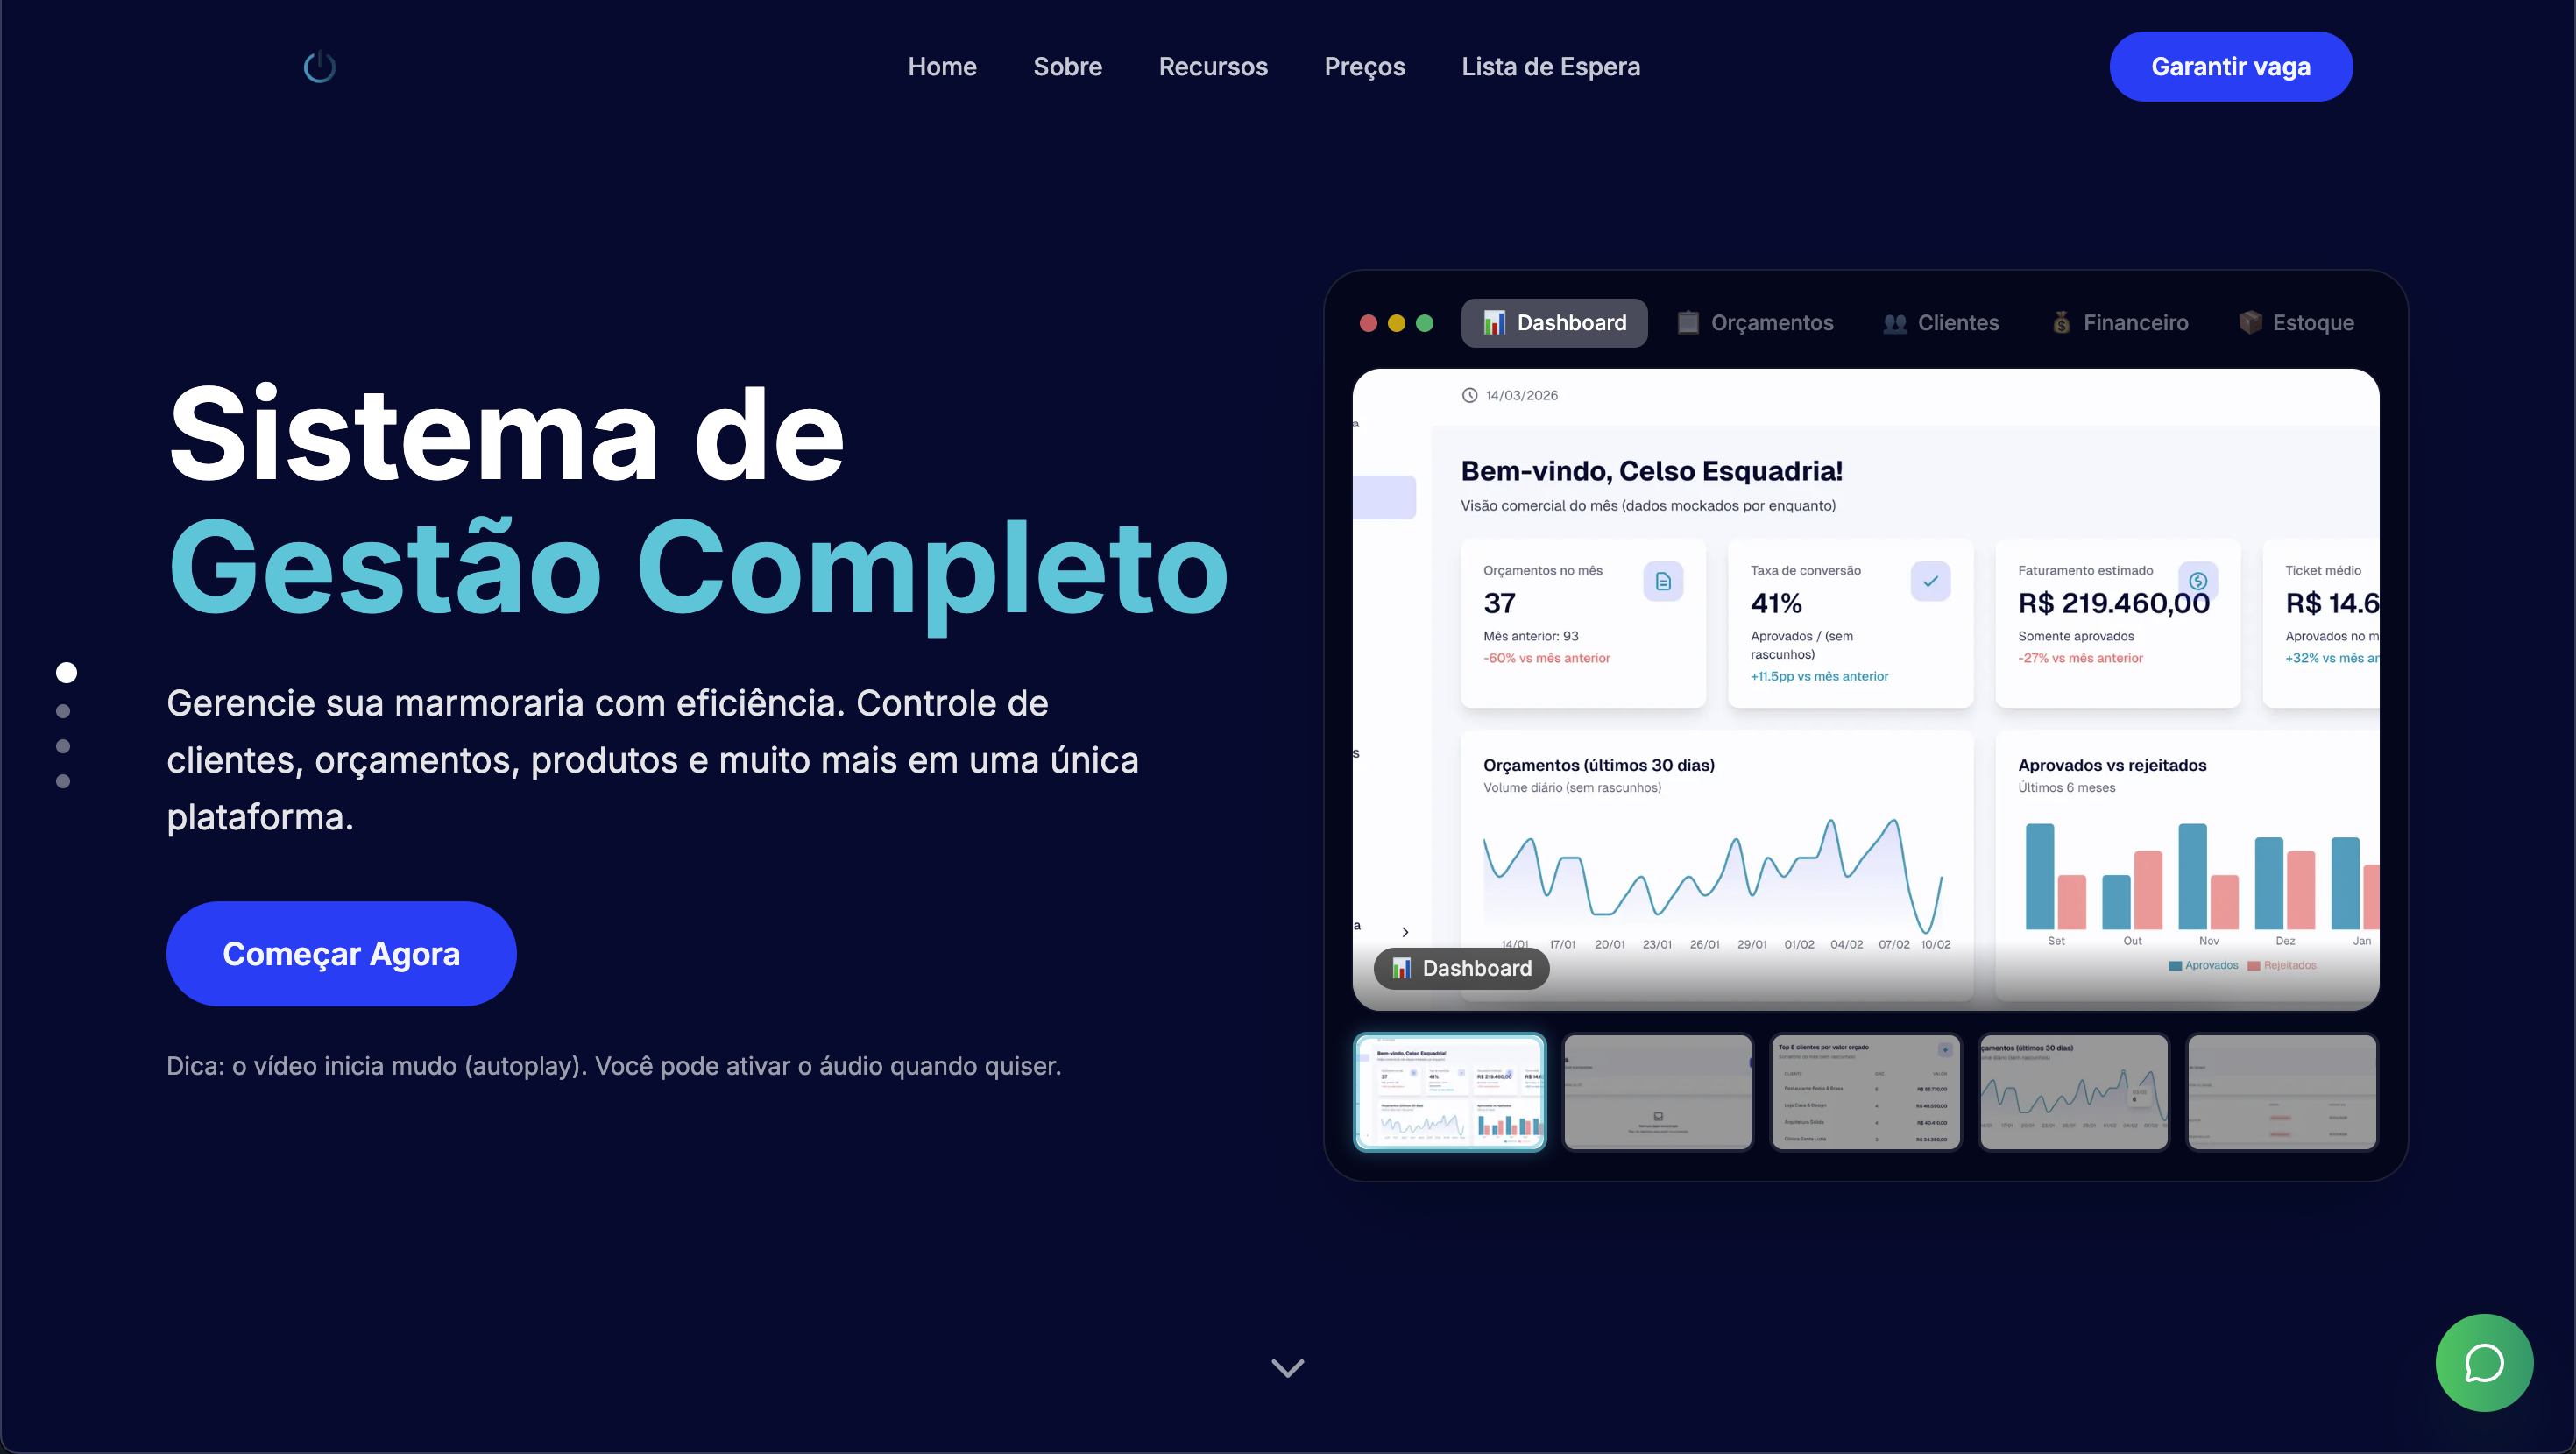
\includegraphics[width=0.95\textwidth]{figures/landing-page.png}
  \label{fig:landing-page}
\end{figure}
{\centering\small Fonte: O Autor, 2026.\par}
\vspace{0.8em}

A seção de planos na landing descreve uma diferenciação futura por porte da marmoraria; nesta fase acadêmica o acesso ao ERP permanece aberto para demonstração, sem cobrança nem limitação de funcionalidades por assinatura.

\subsection{GHCR e GitHub Actions (entrega contínua)}

O GHCR armazena as imagens Docker da API. O GitHub Actions, a cada \textit{push} na ramificação principal, constrói a imagem e a publica no GHCR; a etapa de \textit{deploy} em uma VM ou VPS está implementada e versionada no pipeline (Seção~\ref{sec:workflow-deploy}), mas permanece preparada para quando a operação em nuvem for retomada, não sendo executada de forma contínua nesta fase de validação acadêmica (Capítulo~\ref{cap5Discussao}). Essa integração não se confunde com o armazenamento de mídias do usuário, resolvido pelo backend local descrito na Seção~\ref{sec:testes-e-validacao-cap3} e nesta seção.

O trecho a seguir resume a etapa de implantação do \textit{workflow} do GitHub Actions (\texttt{.github/workflows/deploy.yml}), prevista para ser executada a cada \textit{push} na ramificação principal do repositório da API, após a construção e publicação da imagem no GHCR. O trecho ilustra a sincronização de configuração, o \textit{deploy}, o \textit{health check} e a reversão automática em caso de falha; conforme discutido no Capítulo~\ref{cap5Discussao}, essa etapa está implementada e foi validada em ambiente local, mas não foi exercitada de forma contínua contra uma instância de nuvem pública nesta fase acadêmica.
\label{sec:workflow-deploy}

\begin{verbatim}
export GHCR_OWNER='<owner>'
export IMAGE_TAG='<sha-do-commit>'
PREVIOUS_TAG="$(cat .deployed_tag 2>/dev/null || echo latest)"

docker compose -f docker-compose.prod.yml pull
docker compose -f docker-compose.prod.yml up -d

# health check com nova tentativa, seguido de rollback automático
# para PREVIOUS_TAG caso o endpoint /health nao responda com sucesso
if ! curl -fsSk -H "Host: api.exemplo.com.br" \\
     https://localhost/health; then
  export IMAGE_TAG="$PREVIOUS_TAG"
  docker compose -f docker-compose.prod.yml up -d
  exit 1
fi

echo "$IMAGE_TAG" > .deployed_tag
\end{verbatim}

